%!TEX TS-program = xelatex
%!TEX encoding = UTF-8 Unicode


\documentclass[11pt,twocolumn]{article}
\usepackage{geometry}
\usepackage{indentfirst}
\usepackage{authblk}
\usepackage{url}
\usepackage{graphicx}
\usepackage{subfigure}
\usepackage{amsmath}

%\DeclareGraphicsExtensions{.pdf,.png,.jpg}

\geometry{letterpaper}


\usepackage{fontspec,xltxtra,xunicode}
\defaultfontfeatures{Mapping=tex-text}
\setromanfont{SimSun} %设置中文字体

\XeTeXlinebreaklocale “zh”
\XeTeXlinebreakskip = 0pt plus 1pt minus 0.1pt %文章内中文自动换行


\newfontfamily{\H}{SimHei}
\newfontfamily{\E}{Arial}  %设定新的字体快捷命令
\title{\H 基于CUDA的稀疏矩阵-向量乘法的实现}

\author{吴振伟 (14060050)}
%\affil{计算机学院学员五队}
\date{}
%\date{\E\today}


\begin{document}
\maketitle

\renewcommand\abstractname{摘 要}
\begin{abstract}
稀疏矩阵-向量乘法(SpMV)是科学计算领域的一个基础问题。
因此,高效实现SpVM,对于提升科学计算问题求解性能至关重要。以GPU作为协处理单元提升计算机系统
并行数据处理能力的技术,今年来收到广泛关注。

本文对使用GPU加速SpVM求解的技术进行了系统学习和总结。\\
\end{abstract}

\noindent{\bf 关键词:} SpMV, GPU, CUDA

\section{引言}
众多科学计算问题,如线性方程组求解、偏微分方程求解等,均以稀疏矩阵-向量乘法(SpMV)为基础。高效实现SpMV,长期以来备受关注。

受限于工艺水平、材料物理特性、功耗等因素,单处理机性能提升达到极限。Intel, AMD等主流处理器厂商,均采用多核并行处理的技术,来提高处理器的整体运算性能。相应的,通过并行数据处理对大规模科学运算问题的优化,成为主流技术。

近年来,以通用图形处理单元(GPGPU)作为协处理部件,协同中央处理器(CPU)加速计算机系统对计算密集型程序的执行速度,引起了人们的广泛关注。
在市场需求的驱使下,传统的可编程图形处理单元(GPU)逐步发展成为具有强大运算能力和高度并行性的处理单元。GPGPU是指对图形处理器强大的并行
处理能力和可编程流水线加以利用,协助中央处理器对非图形数据进行处理,即利用GPU对非图形相关的通用计算任务进行加速。

与CPU有所不同,GPU所采用的设计专门面向于具有高度并行性的数据密集型运算。GPU支持的硬件线程数,要远远大于多核CPU支持的硬件线程数。同一段程序在多组数据上并行执行,大大降低了运算过程的控制复杂性,并能够通过数据运算来隐藏访存延迟。这使得在GPU设计中,更多的硬件资源被专用于进行数据处理,而非用于数据缓存和程序流控制;使得GPU拥有相比CPU更加大的浮点运算能力和更高的存储器带宽。

NVIDIA公司于2007年提出了统一计算架构(Compute Unified Device Architecture, CUDA)~\cite{Nickolls:2008:SPP:1365490.1365500},该架构提供了一个清晰的GPU编程模型。
开发者可以基于CUDA,更加高效、充分地利用GPU的运算能力,对通用计算任务进行加速~\cite{Applications}。

本文接下来将分别对GPU和CUDA的架构进行简要介绍;并对基于CUDA编程模型,利用GPU加速大规模稀疏矩阵-向量乘法求解的相关工作,进行对比和总结。

\renewcommand{\figurename}{图}
\section{GPU硬件逻辑结构}
常见的多核心CPU的核数从几个到几十个不等,所支持的并发硬件线程数,在几个到几百个这样一个数量级。而常见的GPU器件,核心数达到几千个,并发硬件线程数远远超过CPU。GPU采用了一些特殊的设计和技术,来调度和管理如此大规模的并发线程。为了加深对GPU硬件结构的认识,这里不失一般性,以Nvidia公司开发的Fermi GPU微体系结构,如图~\ref{fig:fermi} ,对GPU的硬件逻辑结构进行简要的介绍~\cite{Fermi}。
\begin{figure}
  \centering
    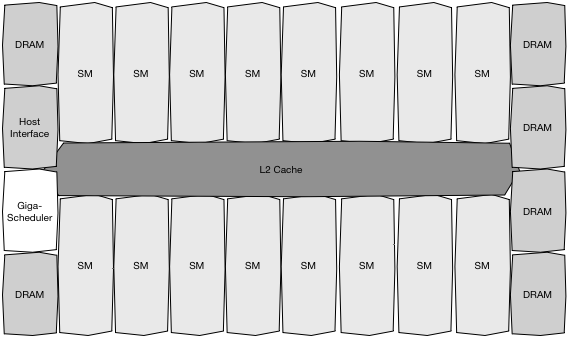
\includegraphics[scale=0.36]{images/hw-layout.png}
  \caption{Fermi微体系结构示意图}
  \label{fig:fermi}
\end{figure}

\begin{figure}
  \centering
    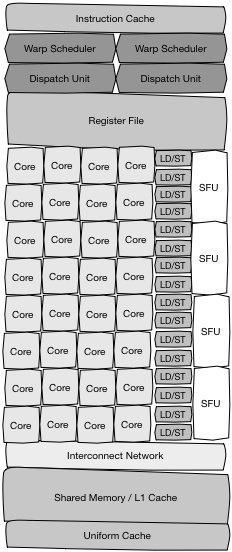
\includegraphics[scale=0.36]{images/sm-layout.png}
  \caption{多线程流处理器结构示意}
  \label{fig:sm-layout}
\end{figure}
GPU构建在一个多线程流式多核处理器(Streaming Multi-processors, SM)阵列之上。如图~\ref{fig:sm-layout}所示,每个SM又由32个处理器核心组成,即最大可以支持32个线程同时运行。在运行时,由GigaSchedular模块负责对任务进行粗粒度的调度——面向SM进行线程调度;SM中的WrapSchedular则负责更细粒度的调度——面向SM中的处理器核心进行线程调度。在下一小节中,本文将结合CUDA编程模型,分别对这两个粗粒度、和细粒度的调度过程,进行更加具体的描述。
%They guide the programmer to partition the problem into coarse sub-problems that can be solved independently in parallel by blocks of threads, and each sub-problem into finer pieces that can be solved cooperatively in parallel by all threads within the block.

\section{CUDA编程模型}
CUDA将线程抽象分组抽象为3个级别:由32个thread组成一个wrap;若干个wrap组成一个block;若干个block进而组成一个grid.

CUDA采用这样一种多层级、嵌套式的方式组织线程,获得了一种对软件开发过程透明的可扩展性。GPU以block为单位,对线程进行粗粒度调度:任意一个block可以被调度到任意一个可用的GPU内部的SM上运行。在SM内部,WrapSchedular又针对被调度的block中的若干个wrap,进行细粒度的调度。
在软件开发过程,编程人员通过上述线程组织结构对计算任务拆分进行描述。
这样一来,在CUDA框架下编写的程序,可以动态适应拥有任意处理器核心数的GPU。

GPU内部的SM,被设计成为SIMT(Single Instruction Multi-Thread)结构。在SIMT结构下,处理器以wrap为最小单位对线程进行调度和管理。当一个wrap被调度时,它所包含的32个thread从同一条指令开始执行;而每个thread拥有其独立的程序计数器和寄存器,所以同一个wrap中的多个thread可以自由进行分支跳转,相互独立地运行。在无跳转发生时,同一wrap中的所有thread共享执行路径;在有跳转发生时,处理器先后串行执行处于不同执行路径上的thread,直至所有分支路径最后又收敛到同一执行路径。忽略SIMT的这些处理细节,是可以保证程序的正确性的。而基于SIMT结构的这些特点,在编写thread代码时,有意识地规避掉执行路径出现分歧的情况,是提高程序性能的一个很好的切入点。
%Not all of the thousands or millions of threads actually run in parallel, but many do. Specifically, an NVIDIA GPU contains several largely independent processors called "Streaming Multiprocessors" (SMs), each SM hosts several "cores", and each "core" runs a thread.

\section{基于CUDA实现SpMV}
针对稀疏矩阵中多数元素为0的这一特点,往往采用压缩存储的方式,实现更高效的存储。本节后续部分,将对几种常见的压缩方式如CSR、ELL等进行简要介绍。

基于CUDA编写的GPU并行程序,可以分为运行在CPU上的串行部分,和运行在GPU上的并行部分。往往以host代指CPU,以device代指GPU.运行在GPU上的线程,被称为kernel.将一个计算任务划分成若干个可以并行执行的子任务的过程,主要体现在对kernel的编写上。

\subsection{几种典型的稀疏矩阵存储格式}
\subsubsection{DIA}
\begin{figure} 
  \centering 
  \subfigure{ 
    \label{fig:subfig:a} %% label for first subfigure 
    	$
		A = \begin{bmatrix}
				1 & 7 & 0 & 0         \\[0.3em]
				0 & 2 & 8 & 0         \\[0.3em]
				5 & 0 & 3 & 9         \\[0.3em]
				0 & 6 & 0 & 4
		\end{bmatrix}
		$
		}
  \hspace{3in} 
  \subfigure{ 
    \label{fig:subfig:b} %% label for second subfigure 
    	$
		data = \begin{bmatrix}
				* & 1 & 7         \\[0.3em]
				* & 2 & 8         \\[0.3em]
				5 & 3 & 9         \\[0.3em]
				6 & 4 & *
		\end{bmatrix}
		$
		$
		offsets = \begin{bmatrix}
				-2 & 0 & 1
		\end{bmatrix}
		$
    } 
  \caption{对角矩阵A的DIA表示} 
  \label{fig:DIA} %% label for entire figure 
\end{figure}

针对对角矩阵、分块对角矩阵等非零元素主要集中在主对角线附近区域的稀疏矩阵,
可以使用DIA格式实现高效存储。
如图~\ref{fig:DIA}所示:

DIA表示由data和offsets两部分组成。data矩阵中的一列,对应矩阵A中的一条非全零对角线,向量offsets一次存放了相应列编号相对主对角列编号的偏移量。
由于超对角线和次对角线上的元素少于主对角线元素,data矩阵中的相应列会出现空缺,应对的方案是分别在次对角线列和超对角线列的头部和尾部添加无关元素。
这样做是为了使data中非零元的行坐标与A中保持一致,非零元的列坐标可以由行坐标加偏移量获得,进一步提高了存储效率。
\subsubsection{ELL}
\begin{figure} 
  \centering 
  \subfigure{ 
    \label{fig:subfig:a} %% label for first subfigure 
    	$
		A = \begin{bmatrix}
				1 & 7 & 0 & 0         \\[0.3em]
				0 & 2 & 8 & 0         \\[0.3em]
				5 & 0 & 3 & 9         \\[0.3em]
				0 & 6 & 0 & 4
		\end{bmatrix}
		$
		}
  \hspace{3in} 
  \subfigure{ 
    \label{fig:subfig:b} %% label for second subfigure 
    	$
		data = \begin{bmatrix}
				1 & 7 & *         \\[0.3em]
				2 & 8 & *         \\[0.3em]
				5 & 3 & 9         \\[0.3em]
				6 & 4 & *
		\end{bmatrix}
		$
		$
		indices = \begin{bmatrix}
				0 & 1 & * \\[0.3em]
				1 & 2 & * \\[0.3em]
				0 & 2 & 3 \\[0.3em]
				1 & 3 & * 
		\end{bmatrix}
		$
    } 
  \caption{对角矩阵A的ELL表示} 
  \label{fig:subfig} %% label for entire figure 
\end{figure}



\subsubsection{COO}
\begin{figure} 
  \centering 
  \subfigure{ 
    \label{fig:subfig:a} %% label for first subfigure 
    	$
		A = \begin{bmatrix}
				1 & 7 & 0 & 0         \\[0.3em]
				0 & 2 & 8 & 0         \\[0.3em]
				5 & 0 & 3 & 9         \\[0.3em]
				0 & 6 & 0 & 4
		\end{bmatrix}
		$
		}
  \hspace{3in} 
  \subfigure{ 
    \label{fig:subfig:b} %% label for second subfigure 
    	$
		row = \begin{bmatrix}
				0 & 0 & 1 & 1 & 2 & 2 & 2 & 3 & 3 &
		\end{bmatrix}
		$
    }
  \subfigure{ 
    \label{fig:subfig:c} %% label for second subfigure 
    	$
		col = \begin{bmatrix}
				0 & 1 & 1 & 2 & 0 & 2 & 3 & 1 & 3 &
		\end{bmatrix}
		$
    }
  \subfigure{ 
    \label{fig:subfig:d} %% label for second subfigure 
    	$
		data = \begin{bmatrix}
				1 & 7 & 2 & 8 & 5 & 3 & 9 & 6 & 4 &
		\end{bmatrix}
		$
    } 
  \caption{对角矩阵A的COO表示} 
  \label{fig:subfig} %% label for entire figure 
\end{figure}
\subsubsection{CSR}
\begin{figure} 
  \centering 
  \subfigure{ 
    \label{fig:subfig:a} %% label for first subfigure 
    	$
		A = \begin{bmatrix}
				1 & 7 & 0 & 0         \\[0.3em]
				0 & 2 & 8 & 0         \\[0.3em]
				5 & 0 & 3 & 9         \\[0.3em]
				0 & 6 & 0 & 4
		\end{bmatrix}
		$
		}
  \hspace{3in} 
  \subfigure{ 
    \label{fig:subfig:b} %% label for second subfigure 
    	$
		ptr = \begin{bmatrix}
				0 & 2 & 4 & 7 & 9 &
		\end{bmatrix}
		$
    }
  \subfigure{ 
    \label{fig:subfig:c} %% label for second subfigure 
    	$
		indices = \begin{bmatrix}
				0 & 1 & 1 & 2 & 0 & 2 & 3 & 1 & 3 &
		\end{bmatrix}
		$
    }
  \subfigure{ 
    \label{fig:subfig:d} %% label for second subfigure 
    	$
		data = \begin{bmatrix}
				1 & 7 & 2 & 8 & 5 & 3 & 9 & 6 & 4 &
		\end{bmatrix}
		$
    } 
  \caption{对角矩阵A的CSR表示} 
  \label{fig:subfig} %% label for entire figure 
\end{figure}
\subsubsection{Hybrid}
\subsection{}

\section{总结}

\renewcommand\refname{引用}
\bibliographystyle{ieeetr}
\bibliography{references}{}


\end{document}